\documentclass[landscape,a0,final]{a0poster}
\usepackage[dvipsnames,svgnames]{xcolor}
\usepackage{tikzposter} % here most of the things are defined
% change parameters only after this line You can also start a new column with an arbitrary 
% x-coordinate by specifying explicitly the coordinate of the new block node as follows:
% not needed:
\usepackage[czech]{babel}
\usepackage[utf8]{inputenc}
\usepackage{wrapfig}
\usepackage{url}

\usepackage[margin=\margin cm, paperwidth=197cm, paperheight=100cm]{geometry}

% \setbackgrounddarkcolor{ForestGreen!70!black}
% \setbackgroundlightcolor{YellowGreen!90!}

% \setfirstcolor{YellowGreen!80!}
% \setsecondcolor{gray!80!}
% \setthirdcolor{red!80!black}

\title{\bigskip GRASS GIS Vector State of the Art  -  Gearing towards GRASS GIS 7 \bigskip}
\author{Markus Metz$^1$, Martin Landa$^2$, Anna Petrášova$^3$, Vaclav Petráš$^3$, Yann Chemin$^4$, Markus Neteler$^1$ and The GRASS GIS Development Team\\ \bigskip
$^1$ CRI, FEM, Italy, $^2$ CTU, Czech Republic, $^3$ NCSU, USA, $^4$ IWMI, Sri Lanka}

\usetemplate{1}
\setinstituteshift{1}

\setblocktitleheight{2}
\setblockspacing{1}

\begin{document}
\ClearShipoutPicture
\AddToShipoutPicture{\BackgroundPicture}
\noindent
\tikzstyle{every picture}+=[remember picture]
\begin{tikzpicture}
\initializesizeandshifts
\titleblock{123.8}{1}
% \setblocktitleheight{1}

\addlogo[north west]{(2,-1)}{9cm}{./svg_images/Grass_GIS.pdf}
%Please insert your institution logo here
\addlogo[north east]{(-2,-2.5)}{4cm}{./svg_images/logo_FEM_CRI.pdf}
\addlogo[north east]{(-2,-6.5)}{4cm}{./svg_images/IWMI_logo.pdf}
\addlogo[north east]{(-8,-2.5)}{4cm}{./svg_images/IWMI_logo.pdf}
\addlogo[north east]{(-8,-6.5)}{4cm}{./svg_images/IWMI_logo.pdf}

%%%%%%%%%%%%%%%%%%%%%%%%%%%%%%%%%%%%%%%%%%%%%%%%%%%%%%%%%%%%%%%%%%%%%%%%%%%%%%%%
\blocknode{Abstract}{
\small The upcoming GRASS GIS 7 release improves not only raster processing and general design but the vector processing in the first place. GRASS GIS, as a topological GIS, recognizes that the topology plays the key role in the vector processing and analysis.\newline
Topology ensures that adjacent geographic components in a single vector map are related. In contrast to non-topological GIS, a border common to two areas exists only once and is shared between the two areas. Topological representation of vector data helps to produce and maintain vector maps with clean geometry as well as enables the user to perform certain analyses that can not be conducted with non-topological or spaghetti data. Non-topological vector data are automatically converted to a topological representation upon import. Further more, various cleaning tools exist to remove non-trivial topological errors.\newline
In the upcoming GRASS GIS 7 release the vector library was particularly improved to make it faster and more efficient with an improved internal vector file format. This new topological format reduces memory and disk space requirements, leading to a generally faster processing. Opening an existing vector requires less memory providing additionally support for large files. The new spatial index performs queries faster (compared to GRASS GIS 6 more than 10 times for large vectors). As a new option the user can select a file-based version of the spatial index for large vector data. All topological cleaning tools have been optimized with regard to processing speed, robustness, and system requirements.\newline
The topological engine comes with a new prototype for direct read/write support of Simple Features API/OGR. \newline
Additionally vector data can be directly exchanged with topological PostGIS 2 databases.\newline
Considering the wide spread usage of ESRI Shapefile, a non-topological format for vector data exchange, it is particularly advantageous that GRASS GIS 7 offers advanced cleaning tools.\newline
For power users and programmers, the new Python interface allows to directly access functions provided by the underlying C library; this combines the ease of writing Python scripts with the power of optimized C functionality in the library backend.
}

%%%%%%%%%%%%%%%%%%%%%%%%%%%%%%%%%%%%%%%%%%%%%%%%%%%%%%%%%%%%%%%%%%%%%%%%%%%%%%%%
\blocknode{Linear features extraction}{
\small
blabla
\begin{center}
 %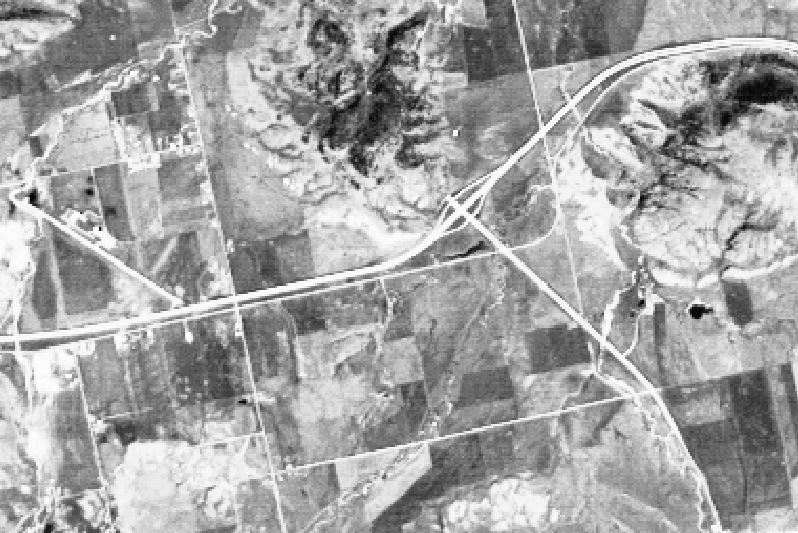
\includegraphics[width=0.48\textwidth]{./images/imagery_spot_original}
 %\hspace{10mm}
 %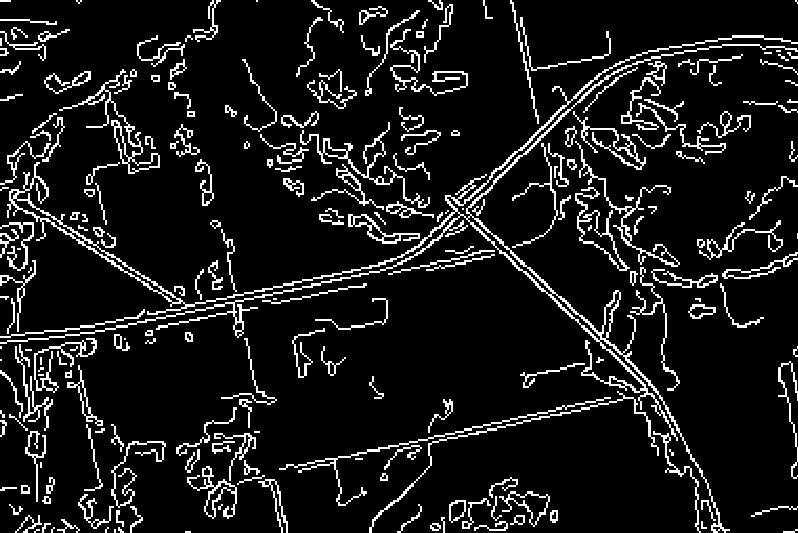
\includegraphics[width=0.48\textwidth]{./images/imagery_spot_edge_1}
 %\newline
 Figure 1: Canny edge detector on a road network [2]
\end{center}
}


%%%%%%%%%%%%%%%%%%%%%%%%%%%%%%%%%%%%%%%%%%%%%%%%%%%%%%%%%%%%%%%%%%%%%%%%%%%%%%%%
\getcurrentrow{box}
\coordinate (funkcionalita) at (box.south west);
\coordinate (funkcionalitaeast) at (box.east);
\coordinate (screenshot) at (box.north west);

\blocknodew[($(funkcionalita)+(20,-1)$)]{35}{References}{
\scriptsize
\begin{center}
\begin{tabular}{rp{0.9\textwidth}}
[1] & Neteler \& Bowman \&  Landa \& Metz, 2012. Environment \& Modeling Software, 31:124-130\\{}
[2] & Petráš, 2012. M.Sc. Thesis, OSGeoREL, FCE CTU, Prague.\\{}
[3] & Kratochvílová \& Petráš, 2013. OSGeoREL, FCE CTU, Prague.\\{}
[4] & Neteler \& Grasso \& Michelazzi \& Miori \& Merler \& Furlanello, 2005. 
International Journal of Geoinformatics, 1(1): 51-61.
\end{tabular}
\end{center}
\smallskip
\hrulefill
\vspace{-5pt}

\begin{center}
\begin{tabular}{cp{0.9\textwidth}}
\begin{minipage}{0.15\textwidth}

\includegraphics[width=0.7in]{./images/iwmi_qr.pdf}
\end{minipage}

\begin{minipage}{0.3\textwidth}
\small {\url{www.iwmi.org}}
\end{minipage}

\begin{minipage}{0.15\textwidth}

\includegraphics[width=0.7in]{./images/grass_qr.pdf}
\end{minipage}

\begin{minipage}{0.3\textwidth}
\small {\url{grass.osgeo.org}}
\end{minipage}
\end{tabular}
\end{center}

\hrulefill
\vspace{14pt}
\begin{center}
\newcommand{\logowidth}{5em}
\newcommand{\logospace}{\hspace{0.1em}}
\noindent

\includegraphics[width=\logowidth]{./svg_images/public_domain_logo.pdf}
\raisebox{0.7\height}{\logospace 2014 GRASS Development Team}
\end{center}
}

\startsecondcolumn

%%%%%%%%%%%%%%%%%%%%%%%%%%%%%%%%%%%%%%%%%%%%%%%%%%%%%%%%%%%%%%%%%%%%%%%%%%%%%%%%
\blocknode{Interactive supervised classification}{
This
\begin{center}
 %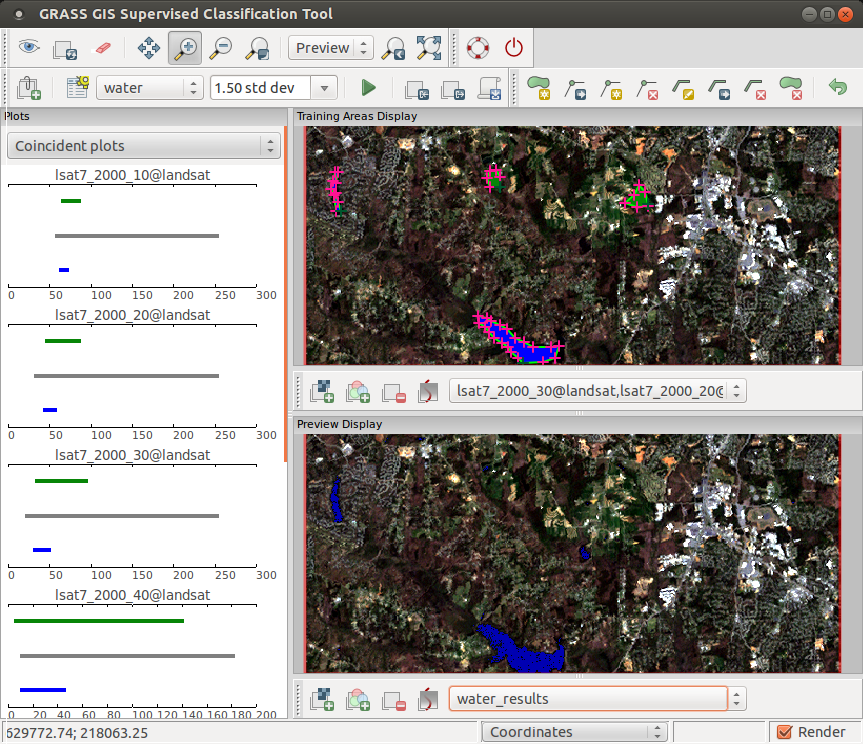
\includegraphics[width=0.47\textwidth]{./images/wxiclass1.png}
 %\newline
 Figure 3: Interactive image classification with coincidence plots (left side) \& histograms (right side)
\end{center}
}

%%%%%%%%%%%%%%%%%%%%%%%%%%%%%%%%%%%%%%%%%%%%%%%%%%%%%%%%%%%%%%%%%%%%%%%%%%%%%%%%
\blocknode{Satellite imagery products}{
blabla
}

\startthirdcolumn
%%%%%%%%%%%%%%%%%%%%%%%%%%%%%%%%%%%%%%%%%%%%%%%%%%%%%%%%%%%%%%%%%%%%%%%%%%%%%%%%
\blocknode{Lidar}{
\smallskip
The Lidar library ({\url {www.liblas.org}}) included in GRASS GIS permits the import of Lidar (.las)
data in raster (r.in.lidar using statistics of choice) or in vector format (v.in.lidar). 
Author Markus Metz tested r.in.lidar with a 705Gb .las file. \newline
On-farm water storage study with lidar data in NSW (Australia) developed a full remote sensing monitoring methodology
of water availability with lidar-based bathymetric survey and multi-source remote sensing survey [8].\newline
\begin{center}
 %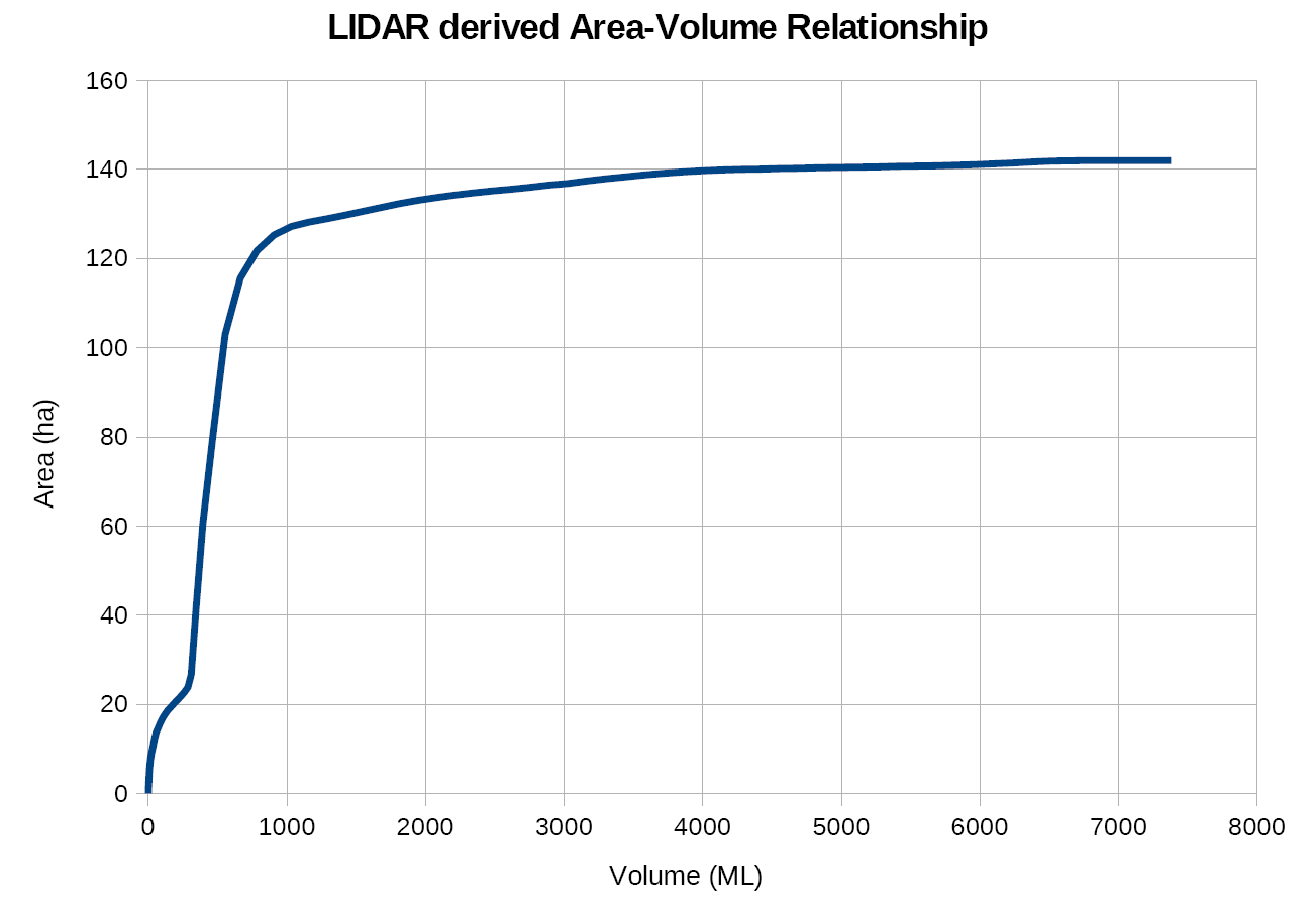
\includegraphics[width=0.4\textwidth]{./images/ofs1}
 %\newline
 Figure 5: On-Farm-Water-Storage Lidar survey and Depth-Volume-Area surveying [8]
\end{center}
}

\blocknode{Other Improvements \& Additions}{
\smallskip

{\bf Remanufacturing, performance improvement}


{\bf Other functions}

\begin{itemize}
 \item {\bf v.} blabla
 \item {\bf v.} blabla
 \item {\bf v.} blabla
 \item {\bf v.} blabla
 \item {\bf v.} blabla
\end{itemize}
}

\startfourthcolumn
%%%%%%%%%%%%%%%%%%%%%%%%%%%%%%%%%%%%%%%%%%%%%%%%%%%%%%%%%%%%%%%%%%%%%%%%%%%%%%%%
\blocknode{Multi- and hyperspectral data analysis}{
\smallskip
Unmixing 

\begin{center}
 %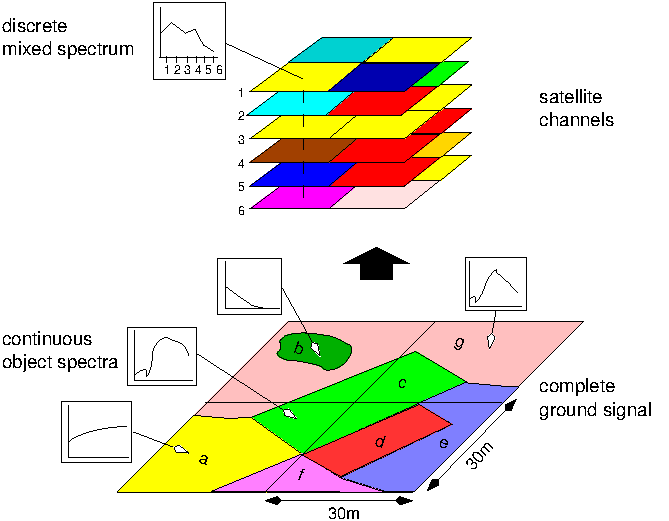
\includegraphics[width=0.4\textwidth]{./images/unmix_pixels_spectrum.pdf}
 %\newline
 Figure 7: Unmixing principle (left), end-members selection (right), error space (below)
\end{center}
}

\end{tikzpicture}

\end{document}
